% Use only LaTeX2e, calling the article.cls class and 12-point type.

\documentclass[12pt]{article}

% Users of the {thebibliography} environment or BibTeX should use the
% scicite.sty package, downloadable from *Science* at
% www.sciencemag.org/about/authors/prep/TeX_help/ .
% This package should properly format in-text
% reference calls and reference-list numbers.

\usepackage[sort]{scicite}
\usepackage{times}
\usepackage{graphicx}
\usepackage{lineno}
\usepackage{color}
\usepackage{multirow}

% The following parameters seem to provide a reasonable page setup.

\topmargin 0.0cm
\oddsidemargin 0.2cm
\textwidth 16.5cm 
\textheight 21cm
\footskip 1.0cm

\usepackage[
  breaklinks=true,
  colorlinks=true,
  linkcolor=blue,anchorcolor=blue,
  citecolor=blue,filecolor=blue,
  menucolor=blue,pagecolor=blue,
  urlcolor=blue]{hyperref}
  
%The next command sets up an environment for the abstract to your paper.

\newenvironment{sciabstract}{%
\begin{quote} \bf}
{\end{quote}}


% If your reference list includes text notes as well as references,
% include the following line; otherwise, comment it out.

%\renewcommand\refname{References and Notes}

% The following lines set up an environment for the last note in the
% reference list, which commonly includes acknowledgments of funding,
% help, etc.  It's intended for users of BibTeX or the {thebibliography}
% environment.  Users who are hand-coding their references at the end
% using a list environment such as {enumerate} can simply add another
% item at the end, and it will be numbered automatically.

\newcounter{lastnote}
\newenvironment{scilastnote}{%
\setcounter{lastnote}{\value{enumiv}}%
\addtocounter{lastnote}{+1}%
\begin{list}%
{\arabic{lastnote}.}
{\setlength{\leftmargin}{.3in}}
{\setlength{\labelsep}{.5em}}}
{\end{list}}


% Include your paper's title here

\title{The Spatial and Temporal Domains of Modern Ecology }%\\
%OR Ecology's Spatio-temporal Domains\\
%OR Space, Time, and Ecology \\
%OR Ecology: still a small-scale, field-based discipline} 
 
\author
{Lyndon Estes$^{\ast1, 2}$, Paul R. Elsen$^{3, 4}$, Tim Treuer$^{4}$, Labeeb Ahmed$^{5}$, \\
Kelly Caylor$^{6, 7}$, Jason Chang$^{5}$, Jonathan J. Choi$^{8}$, and Erle Ellis$^{5}$ \\
\\
\normalsize{$^{1}$Graduate School of Geography, Clark University, Worcester MA 01610, USA}\\
\normalsize{$^{2}$Woodrow Wilson School, Princeton University, Princeton, NJ 08544, USA}\\
\normalsize{$^{3}$Department of Environmental Science, Policy, and Management,}\\
\normalsize{University of California Berkeley, Berkeley, CA 94720, USA}\\
\normalsize{$^{4}$Ecology and Evolutionary Biology, Princeton University, Princeton, NJ 08544, USA}\\
\normalsize{$^{5}$Geography and Environmental Systems, University of Maryland Baltimore County,}\\ 
\normalsize{Baltimore, MD 21250, USA}\\
\normalsize{$^{6}$Department of Geography, University of California Santa Barbara, Santa Barbara, CA 93106, USA}\\
\normalsize{$^{7}$Bren School of Environmental Science and Management,}\\
\normalsize{University of California Santa Barbara, Santa Barbara, CA 93106, USA}\\
\normalsize{$^{8}$Nicholas School of the Environment, Duke University, Durham, NC 27708, USA}\\
\normalsize{$^\ast$To whom correspondence should be addressed; E-mail:  LEstes@clarku.edu.}}
% Include the date command, but leave its argument blank.

\date{}


%%%%%%%%%%%%%%%%% END OF PREAMBLE %%%%%%%%%%%%%%%%

\begin{document} 

% Double-space the manuscript.

\baselineskip12pt

% Make the title.

\maketitle 

\section*{Abstract}
\textbf{To understand ecological phenomena, it is necessary to observe their behavior across multiple spatial and temporal scales. Since this need was first highlighted in the 1980s, technology has opened previously inaccessible scales to observation. To help determine whether there have been corresponding changes in the scales observed by modern ecologists, we analyzed the resolution, extent, interval, and duration of observations (excluding experiments) in 348 studies published between 2004-2014. We found that observational scales were generally narrow because ecologists still primarily use conventional field techniques. In the spatial domain, most observations had resolutions $\leq$1 m$^2$ and extents $\leq$10,000 ha. In the temporal domain, most observations were either unreplicated or infrequently repeated ($>$1 month interval), and $\leq$1 year in duration. Compared to studies conducted prior to 2004, observational durations and resolutions appear largely unchanged, but intervals have become finer and extents larger. We also found a large gulf between the scales at which phenomena are actually observed, and the scales those observations ostensibly represent, raising concerns about observational comprehensiveness. Furthermore, most studies did not clearly report scale, suggesting that it remains a minor concern. Ecologists can better understand the scales represented by observations by incorporating autocorrelation measures, while journals can promote attentiveness to scale by implementing scale reporting standards.}

%\linenumbers
\vspace{10pt}
\noindent \textbf{Introduction}
\vspace{5pt}
\\
The scales at which ecosystems are observed play a critical role in shaping our understanding of their structure and function \cite{levin_problem_1992,chave_problem_2013,wiens_spatial_1989}.  Ecological patterns emerge from temporal and spatial domains that may be coarser or finer than the processes that shape them, which means that investigation across multiple scales is essential for understanding ecological phenomena \cite{levin_problem_1992,sandel_scale_2009}. This awareness has grown rapidly since the 1980s, accelerated by the need to understand how changes in the global climate, ocean, and land systems are affecting everything from individual populations \cite{tingley_push_2012} to entire biomes \cite{xiao_photosynthetic_2004}, while technological advances in areas such as remote sensing and genetics are making it ever-easier to quantify ecological features across a broad and increasing range of scales \cite{schneider_rise_2001, chave_problem_2013}.  

Given the growing awareness of scale, expanding data gathering capabilities, and the fact that the most comprehensive (and arguably best-known) meta-analyses \cite{tilman_ecological_1989,kareiva_spatial_1988} of ecological research scales were published nearly 30 years ago (but see \cite{porter_crop_2005,sandel_scale_2009} for more recent reviews), it is both timely and important to assess the scales of contemporary ecological investigation. To address this need, we quantified the spatial and temporal domains of empirical observations that were reported within recently (2004-2014) published ecological studies. We define domain as the distribution of observations within the spectrum of one or more scale dimensions\footnote{This definition differs slightly from Wiens' \cite{wiens_spatial_1989}, who defined ``domain of scale'' as ``a portion of the scale spectrum within which process-pattern relationships are consistent regardless of scale.''}, and empirical observations as ecological observations collected under un-controlled or non-manipulated conditions. Empirical observations are critical for developing and testing the models that explain why ecological patterns vary in time and space \cite{levin_problem_1992, tilman_ecological_1989}, therefore the spatio-temporal domains of observations provide an important indicator of the field's progress towards achieving a holistic, predictive understanding of ecosystems \cite{chave_problem_2013,levin_problem_1992}. 

Our study focused on two dimensions of spatial scale, resolution (grain) and extent, and two of temporal scale, interval and duration (Table 1). We analyzed the observational domains within each of these four dimensions and between pairs of these dimensions. We also assessed two additional dimensions, \emph{actual} extent (the summed area of spatial replicates) and \emph{actual} duration (the summed observational time of temporal replicates), which we used to evaluate how much the actual scales of observation (i.e. how much space and time is covered by the measurement) differ from the scales that they ostensibly represent. These differences may impact how effectively observations characterize ecological phenomena. For one, an increasing gap between actual and ostensible observational scales implies greater interpolation or extrapolation of observed measurements, raising the odds of over-leveraging data. Furthermore, since natural systems are frequently complex, non-linear, and non-random \cite{levin_ecosystems_1998,pringle_spatial_2017,rietkerk_regular_2008}, a larger gap increases the likelihood of data challenges such as censoring (\emph{sensu} \cite{efron_efficiency_1977}), as phenomena may resolve themselves in the space or time between replicates. 

\begin{table}[htp]
\caption{The scale dimensions of ecological observations assessed in this meta-analysis.}
\begin{center}
\begin{tabular}{llll}
\hline
\multicolumn{2}{c}{\textbf{Component}} & \textbf{Units} & \textbf{Description} \\\hline\hline
\multirow{3}*{Spatial} & Resolution & m$^2$ & Area of an individual spatial replicate (e.g. plot) \\%\cmidrule(l){2-3}
   & Extent & ha & Area  encompassed by all spatial replicates \\
   & Actual extent & ha & Summed area of all spatial replicates\\\hline
\multirow{3}*{Temporal} & Interval & days & Time elapsed between successive temporal replicates \\
   & Duration & days & Time elapsed between first and last temporal replicates\\
   & Actual duration & days & Summed observational time of all temporal replicates\\
\hline
\end{tabular}
\end{center}
\label{default}
\end{table}%

\vspace{10pt}
\noindent \textbf{Results}
\vspace{5pt}
\\
We reviewed 348 papers randomly selected from 42,918 titles published between 2004-2014 in the top 30 ecology-themed journals. We extracted scale data from 378 observations of ``natural'' (i.e. non-experimentally manipulated) ecological features reported within 133 of the reviewed papers (plus an additional 62 cited as the source of observations). The majority of sampled observations were collected using conventional field methods (80\%), followed by automated \emph{in situ} sensing techniques (12.4\%), remote sensing (6.9\%), and paleo-reconstruction ($<$0.8\%). 

\vspace{5pt}
\noindent \textbf{\emph{Observational domains within individual dimensions}}\\
In terms of resolution, spatial replicates for the majority (67\%) of observations (across all methods) were $\leq$1 m$^2$, a further 24\% were 1 m$^2$ up to 1 ha, and the remaining 9\% were $>$1 ha (Fig. 1A). These distributions primarily reflect those of field observations, the dominant observational methodology. Examining the distributions for each observational method (Supplementary Figure 1) shows that automated sensing and paleo-reconstruction had resolutions that were generally finer (85\% or more $\leq$0.1 m$^2$) than field observations (47\% $\leq$0.1 m$^2$), while the majority of remote observations were much coarser (70\% $>$100 m$^2$).   

The extent of 19\% of observations was $\leq$10 ha, 23\% covered 10-1,000 ha, 11\% 1,000-10,000 ha, 19\% 10,000-100,000 ha, 12\% 100,000-1,000,000 ha, and 15\% $>$1,000,000 ha (Fig. 1B).  As with resolution, the extent covered by automated sensing methods tended to be smaller (52\% $\leq$100 ha) than those of field observations (31\% $<$100 ha), while all but 4\% of remote observations covered areas $>$10,000 ha (as did the small number of paleo-reconstructions).  

%16 + 29 + 26 + 67 + 14 + 37 + 10

In the temporal dimensions, 37\% of observations were not repeated (Fig. 1C), 17\% were repeated at short intervals (sub-second to daily), 20\% at daily to monthly intervals, 18\% at monthly to yearly intervals, 6\% at yearly to decadal intervals, and 2\% at decadal or greater intervals. Among temporally replicated observations (Supplementary Figure 1), automated sensing had the finest intervals (61\% $\leq$1 day; 100\% $\leq$1 year), followed by remote observation (37\% $\leq$1 day; 78\% $\leq$1 year), field methods (17\% $\leq$1 day; 86\% $\leq$1 year), and paleo-reconstructions (21\% $\leq$1 decade).   

Duration was $\leq$1 day for 31\% of sampled observations (due to lack of temporal replication), while 10\% covered one day to one month, 23\% one month to one year, 27\% 1-10 years, and 9\% a decade or more (several paleoecological studies covered centuries; Fig. 1D). Paleo-reconstructions naturally had the longest duration (67\% $>$ 1 decade), while just $\sim$40\% of field, automated, and remote observations had durations exceeding one year.

\vspace{5pt}
\noindent \textbf{\emph{Observational domains within two-dimensions}}\\
Contrasting resolution with interval reveals that the majority of temporally replicated observations (unrepeated observations were excluded because they lack intervals) had resolutions of 10 cm$^2$-1 m$^2$ and were revisited at daily to yearly intervals (Fig. 2A). A less dense, oblong concentration of observations bounded on the upper left by monthly to yearly observations at 100 m$^2$ resolution and on the lower right by near-daily to monthly observations with 1-10 ha resolution is also evident. The four observational methods occupied substantially different domains, as indicated by the locations of their median values (and see Supplementary Figure 2): the median domain of field observations had 0.1-1 m$^2$ resolution and a monthly interval, whereas remote observations had a coarser median resolution (1,000 m$^2$) but finer median interval ($\sim$1 day). Paleo-reconstructions and automated sensing techniques were both finely resolved (median between 10 cm$^2$-0.01 m$^2$), but automated approaches had an hourly-daily median interval compared to multi-decadal for paleo-reconstructions. 

Comparing the interval and duration of temporally replicated observations showed most observations had daily to decadal intervals and durations of 1 month to 1 decade (Fig. 2B). The orientation of this concentration shows that interval increases with duration; observations lasting one month to one year tend to have daily to monthly intervals, while those lasting 1 year to 1 decade tend to have yearly to decadal intervals. This tendency is reflected in the domain medians of the primary observational methods: automated sensing had the finest median interval (hour-day) and shortest duration (month-year), followed by remote sensing (median interval slightly greater than one day and median duration of 1 year), field observations (median monthly interval and duration just over 1 year), and finally paleo-reconstructions (median interval 1 decade and millennial duration). 

Contrasting the two spatial dimensions against one another shows a primary concentration of observations of 10 cm$^2$ to nearly 100 m$^2$ resolution with extents ranging between $\sim$1,000-1,000,000 ha (Fig. 2C). The second-most prominent concentration consists of higher resolution (1 cm$^2$-1 m$^2$), smaller extent (10-1,000 ha) observations, beneath which lies a third and fainter concentration of 1-1,000 cm$^2$ resolution and 1000 m$^2$ to $\leq$10 ha extent. These three concentrations suggest that observational extent increases with resolution, which is further evident in the median domain values (and kernel densities; Supplementary Figure 2) of automated (0.01 m$^2$ resolution, 100 ha extent), field (0.1-1 m$^2$ resolution, 1,000-10,000 ha extent), and remote (1,000 m$^2$ resolution, 1-10 million ha extent) observations.  Paleo-reconstructions were an outlier from this relationship, having very fine median resolution (0.01 m$^2$) but large extent (1 million ha), a possible artifact of small sample size. 

There are two primary observational domains within the contrast between duration and extent. The first consists of observations lasting one month to one decade with extents of 10-1,000 ha, while the second is defined by observations of one year to several decades that cover 10,000-1,000,000 ha (Fig. 2D).  Three other notable, but lesser concentrations are also evident, including small area observations (0.1-1 ha) covering one month to decade, and short duration, temporally unreplicated observations ($\leq$1 day) of either 1-100 ha or 10,000-1,000,000 ha.  The median observation from automated sensing (1 year duration, 100 ha extent) lies near the center of the first major concentration, while the median extents of field (1,000-10,000 ha) and remote (1-10 million ha) observations bound the second major concentration at its upper and lower extents, with the median duration of both observational types falling between 1 month to 1 year. 

\vspace{5pt}
\noindent \textbf{\emph{Differences between actual and ostensible scales}}\\
Observational extent was on average 5.6 orders of magnitude larger than actual extent (Fig. 3A). This difference increased with extent, reaching a maximum of 8.3 between 100 million and 1 billion ha of extent, then falling to 3 orders of magnitude between 1-10 billion ha (these extents were covered by $<$2\% of observations, which were primarily collected with remote sensing). Remote observations had the smallest mean difference magnitude (1.9), compared to 5.7 or larger for the other three methods (Supplementary Figure 3). 

The magnitudes of difference between observational duration and actual duration was somewhat smaller, averaging 3.4 and ranging from just under 2 for the shortest durations (hour-day) to over 4 for observations lasting 1 decade to 1 century (Fig. 3B). As with extent, the difference fell substantially for the longest durations (century to millenia), as these domains were covered by paleo-reconstructions (Supplementary Figure 3), which have little difference between actual and ostensible duration because coring techniques capture continuous temporal records. The mean difference magnitudes for the other three observing methods ranged from just over 3 (field and automated sensing) to nearly 6 (remote observations). 

\vspace{5pt}
\noindent \textbf{\emph{Potential biases and uncertainties in quantifying scales}}\\
Our results were potentially influenced by several methodological issues. First, most studies did not precisely report observational scales, thus we had to estimate, rather than simply record, scale values for the majority of observations (we estimated 63, 60, 69, 36, 64, and 83\% of resolution, extent, actual extent, interval, duration, and actual duration values, respectively). Estimation errors may therefore have biased our findings. We attempted to quantify and account for this error by assessing between-observer variability and incorporating this uncertainty into our resampling methodology (Supplementary Results). The resulting confidence intervals (Fig. 1) suggest that that estimation errors did not unduly influence our findings. 

Our scale-estimation protocols may also have introduced bias, particularly our rule for estimating resolution (the smallest areal unit of \emph{complete} measurement). We selected this definition for the sake of consistency, but some papers reported resolution as a larger area in which sub-samples were taken. For these, our estimates were finer than what the studies' authors considered to be the resolution. Our results would also  be somewhat different if we had included observations from experiments. For example, average resolution and duration would likely be finer \cite{tilman_ecological_1989,kareiva_spatial_1988}. Additionally, the token 1 second (Supplemental Methods) we used to represent the duration of remotely sensed temporal replicates (which are effectively instantaneous) caused us to underestimate the differences between their durations and actual durations (Supplementary Figure 3). However, the relatively small number of remote observations suggests that the impact of this bias on our overall findings was negligible.  

It is also possible that our findings misrepresent observational domains because of sampling error. Although we randomized our sample to ensure representativeness, we reviewed just 0.8\% of the papers published during our study period. Our sample may therefore under- or over-represent observational coverage in certain domains, particularly for specific methods. This possibility is greatest for paleo-reconstructions, where the small sample size likely resulted in an overestimate of typical observational extent (e.g. Fig. 2B, C; however, the interval and duration values are probably more representative). 

Finally, our omission of papers published after 2014 could also have biased our findings. Although our sample size was too small to assign statistical significance, we found a possible positive trend in the use of remote observations and a corresponding decline in field observations over the course of our study period. If these trends were not spurious, they suggest that including studies from 2015-2017 would result in a somewhat larger relative sample of remote observations, which would in turn slightly increase the mean extent of ecological observations (see Supplementary Results for further details). 

\vspace{10pt}
\noindent \textbf{Discussion}
\vspace{5pt}
\\
\noindent \textbf{\emph{Insights into the scale domains of modern ecology}}\\
Our results suggest that modern ecology's observational domains are fairly narrow, and that ecologists still primarily rely on conventional field-based observational techniques. In the spatial dimensions, the majority of observations have grains of $\leq$1 m$^2$ and extents of $\leq$10,000 ha (Fig 1A;B). In the temporal dimensions, most observations are either un-replicated or relatively infrequent ($>$1 month interval; Fig. 1C) and have relatively short duration ($\leq$1 year; Fig. 1D). 

Contrasting observational dimensions reveals that larger extents are associated with larger spatial replicates (Fig. 2C), while longer durations are associated with longer intervals (Fig. 2B). The latter association reflects a cost-imposed tradeoff between sampling frequency and temporal duration that is characteristic of field observations, but also appears to affect the other three methods, as evidenced by their relative domain locations. A similar tradeoff can be seen in the inverse relationship between resolution and interval (Fig. 2A), which primarily relates to field observations, where larger spatial replicates demand greater effort, which in turn reduces sampling frequency \cite{kareiva_spatial_1988}. Less obvious is the opposite tradeoff that affects remote observation (Supplementary Figure 2), where finer resolution (which is necessary for detail) typically necessitates longer intervals \cite{estes_platform_2016}.   

As a result of these tradeoffs, there are several notable observational gaps, specifically within the domains defined by high frequency (daily to sub-daily intervals) observations having 1) high to moderate resolutions ($>$1 m$^2$ up to 100 ha; Fig. 2A) and 2) decadal or longer durations (Fig. 2B).  Another hole is evident in the high to moderate resolution, large extent (1 million-10 billion ha) domain (Fig. 2C). 

Have these domains changed since the seminal papers on scale first appeared in the late 1980s \cite{wiens_spatial_1989, levin_problem_1992, tilman_ecological_1989}? A comprehensive answer would require a repeat similar analysis focused on earlier literature, but the data provided by three prior studies provides partial insight.  The first dataset consists of duration values that Tilman \cite{tilman_ecological_1989} extracted from 623 studies published between 1977-1987 in the journal \emph{Ecology}. The mean duration of the most comparable subset of those values (n=419) was 3.6 years, versus 3.3 years in our sample (or 5.1 when excluding temporally un-replicated observations). The second dataset is found in Kareiva and Anderson \cite{kareiva_spatial_1988}, who assessed the resolutions of 97 community ecology experiments published in \emph{Ecology} between 1980-1986. The average of those (12,657 m$^2$) was substantially smaller than the mean of our sample (1,479,465 m$^2$), but comparing Kareiva and Anderson's \cite{kareiva_spatial_1988} 80th percentile value (197 m$^2$) to ours (115 m$^2$) shows that the majority of contemporary observations are finer-grained than most 1980s-era experiments. Porter et al \cite{porter_wireless_2005} provide the third dataset, which compares the extent and interval of 25 studies published in 2003 and 2004 (also in \emph{Ecology}). The mean interval was 178 days, compared to 684 days in our sample, but the 80th percentile value in our study was 169 days compared to 329 days in theirs. Extent in our sample was substantially larger according to multiple summary statistics, including the mean (368,403 ha versus 114,965,072 ha in our study), median (9 ha versus 5,051 ha), and 95th percentile (136,000 ha versus 46,424,808 ha; this value is smaller than the mean, which is skewed by a small number of very large extent observations). 

Although limited due to methodological differences (e.g. a focus on experiments versus un-manipulated systems), these comparisons suggest that the duration and resolution of ecological observations have changed little in the past 30 years, but observational frequency and extent have both increased. A weak positive trend in our own data also suggests that the mean extent of ecological observations is steadily increasing (Supplementary Figure 5), which likely corresponds to increasing use of remote sensing (Supplementary Figure 4). 

Despite this apparent increase in observational extent, there remains a large gulf between the areas that ecologists actually observe and the areas their observations are intended to represent (Fig. 3A). A substantial discrepancy also exists between the amount of time spent observing phenomena and the time spans those observations theoretically represent (Fig. 3B). These differences between the actual and ostensible scales of observation have implications for ecological understanding, as the unobserved portions of space and time may contain important patterns and processes that are not captured by replicates, due to phenomenon-dependent factors such as autocorrelation and representativeness of the sampling scheme \cite{underwood_experiments_1997,palmer_scale_1994, cao_comparison_2002, legendre_spatial_1993,collins_method_2000}. Brief, infrequent snapshots, or fine-grained, spatially sparse replicates, may be sufficient to characterize many phenomena (e.g. annual changes in tree cover are well-represented by low frequency satellite imaging \cite{hansen_high-resolution_2013}), but may be inadequate for more dynamic phenomena. For example, wildfire extent and duration can be mapped by daily return satellites \cite{roy_prototyping_2005,jones_fire_2009}, but the instantaneous nature of the imaging means that it cannot be used to observe fire behavior \cite{clements_observing_2007}. To capture such behavior, long periods of continuous observation may be more important for understanding dynamics than frequent repeats. 

It is therefore important to examine whether the scales of the phenomena being observed are adequately captured by the design of replicates. Our methods suggest one possible procedure for assessing the \emph{scale representativeness} of observations, which is to 1) calculate the autocorrelation (spatial or temporal) within the observations (using a semi-variogram, for example), 2) find the threshold distance (or time) below which a suitably strong correlation (e.g. r=0.7) will exist between neighboring sampled values, 3) add that distance (or time) to the sample resolution (or duration), and 4) recalculate actual extent (or duration) using the adjusted resolution (or sampling duration). The difference between this autocorrelation-adjusted actual extent (or actual duration) and extent (or duration) may provide a useful additional measure of how well the replicates represent the intended scale of observation. Though increasing spatial or temporal coverage may not always be the goal of a study, if the gap between actual and ostensible values remains large, then alternative sampling methods may be used to close it. For example, remote sensing provides wall-to-wall spatial coverage of a study area, erasing the difference between actual extent and extent. Furthermore, the interval of high-resolution imaging (higher resolution is preferred in images as it allows individual features to be better discerned \cite{dark_modifiable_2007, hay_comparison_2003}) is now approaching daily to sub-daily scales \cite{drusch_sentinel-2:_2012, hand_startup_2015}, allowing improved representation of spatial and temporal dynamics. For phenomena that can't be measured from space, either because they are not visible or because they require continuous observation, new approaches for collecting \emph{in situ} or near-surface observations (e.g. low-cost wireless sensors \cite{wolf_gsm-based_2012, collins_new_2006, porter_wireless_2005}, citizen observers \cite{dickinson_current_2012}, and autonomous vehicles \cite{anderson_lightweight_2013}) can be used to increase the spatial and temporal coverage of observations.

The aforementioned insights regarding modern observational domains must be tempered by the uncertainty within our own scale estimates, as detailed in the preceding section. However, most of this uncertainty is attributable to unclear reporting of scale values in the majority of papers we reviewed (a problem also noted in geography studies \cite{margulies_ambiguous_2016}). This tendency towards vague documentation offers one final insight: despite decades of accumulated knowledge regarding its importance \cite{levin_problem_1992, wiens_spatial_1989, chave_problem_2013, wheatley_factors_2009}, scale appears to remain a low priority throughout much of the ecological discipline. Beyond contributing to the broader problem of scientific reproducibility \cite{baker_1500_2016}, inattentiveness to scale increases the risk that observations inadequately represent the phenomenon of interest, thereby limiting the generalizability of any derived ecological knowledge \cite{margulies_ambiguous_2016, wheatley_factors_2009, wiens_spatial_1989}. To mitigate this problem, we recommend that ecological journals require authors to quantify and clearly report the values of resolution, extent, interval, and duration. Fortunately, some journals already appear to be implementing such policies; for example, \emph{Global Ecology and Biogeography} now requires information on the spatial, temporal and taxonomic scale of studies to be in the abstract (a policy adopted in early 2016).

\vspace{5pt}
\noindent \textbf{\emph{Looking forward}}\\
Our study suggests that the concept of scale has yet to fully permeate the discipline of ecology. Evidence for this assertion lies in the continued narrowness of ecology's observational scale domains and the poor documentation of scale dimensions in the literature. However, the increasing extent of ecological observations, enabled by remote sensing and presumably motivated by many ecologists' appreciation of scale-related issues, suggests that ecology's scale domains are gradually changing. In the coming years, the accelerating gains in technology and analytical methods will allow researchers new and unprecedented capabilities to peer into, and thus close, the prominent holes in observational domains. A renewed, discipline-wide focus on scale's importance, including the adoption of stricter scale-reporting standards by journals, will help spur ecologists to address these gaps, while fostering the improved transferability of knowledge within the discipline.  

\vspace{10pt}
\noindent \textbf{Methods}
\vspace{5pt}
\\
\noindent \textbf{\emph{Paper selection and review}}\\
We used the 2012 Web of Science impact factors to select the highest ranked ecology-themed journals that published studies with an observational component, excluding journals devoted to reviews, meta-analyses, laboratory, cellular, or experimental studies.  To select a representative sample of recent ecology studies, we downloaded the metadata for all papers published in the 30 selected journals (Supplementary Table 1) between 2004 and 2014. Our study involved six different observers (those reviewing the papers to extract the observational scales), each of whom was given a randomly selected batch of 500 titles.  A separate set of 20 papers was also randomly selected, and was given to all observers to review independently in order to 1) calibrate the interpretations and extraction of scale-related information between observers, and 2) to estimate between-observer variance.  

Each observer first reviewed the papers in the calibration set, and then commenced reviewing papers in their individual random draws, beginning at the top of the list and then proceeding until at least 20 eligible papers describing ecological observations were reviewed. In cases where the reviewed papers used observations that were described in another publication, we reviewed those source papers in order to extract the observational dimensions. We excluded papers that were opinion or perspectives pieces (unless they presented or used existing observational data), or theoretical studies based on generated data. We also did not collect scale information from papers (or the relevant parts of papers) describing experimental manipulations, because experiments tend to be of limited extent, duration, and resolution due to their higher logistical costs \cite{tilman_ecological_1989, kareiva_spatial_1988}. Including data from experiments would therefore likely have biased our findings towards finer scales, while minimizing the impact that new observing methods (e.g. satellite imaging, wireless sensing) may have had in expanding the scales of ecological investigation \cite{turner_remote_2003,pettorelli_satellite_2014,porter_wireless_2005}. A bibliography of the reviewed papers appears in the Supplementary Information. 

\vspace{5pt}
\noindent \textbf{\emph{Estimating observational scales}}\\
We recorded six primary dimensions of ecological observations, three related to space and three related to time. The space-related dimensions were resolution, extent, and actual extent. Here extent was primarily defined as the area falling within a perimeter defined by the outermost spatial replicates, while actual extent was  the summed area of all spatial replicates (i.e. N * resolution, where N is the number of spatial replicates, which we also recorded), or the area that ecologists observe in practice. In assessing spatial scales, our analysis only considered the Cartesian plane; we did not calculate the z, or depth, dimension, although this dimension is of greater importance for certain sub-disciplines of ecology (e.g. depth profiles in marine ecology). In some cases (primarily paleoecological studies), values extracted from the z-dimension provided temporal information that was used to calculate both the interval and the duration of the observation.  

For time dimensions, we extracted information related to observational interval, duration, and actual duration. Duration was defined as the time between the first and last temporal replicate, whereas actual duration quantifies the amount of time spent observing a particular location, which we calculated by multiplying sampling duration (the time spent collecting a single temporal replicate) by the number of temporal replicates.  

A full definition of all dimensions and how they were recorded is contained within a list of Frequently Asked Questions (FAQ; see Supplementary Methods), which was provided to each observer for initial study and reference, and adapted as necessary during the course of the study, in order to ensure methodological consistency.  

To account for potential differences in scales related to methodology, we classified each observation according to the following broad categories, which were field methods (manual \emph{in situ} data collection), automated (\emph{in situ}) sensing, remote sensing/other geographic data (hereafter remote observations), and paleo-reconstruction approaches. We also recorded when observations were reported in any study with an unclear or missing scale value.  

\vspace{5pt}
\noindent \textbf{\emph{Calibration and consistency}}\\
Most studies did not explicitly report values for all the assessed scales, and thus interpretation and judgement had to be applied to develop reasonable estimates for their values. The FAQ (Supplementary Methods) provided the protocol we followed, and was initially developed following consultation between observers prior to the commencement of review. We conducted an iterative process of calibration to ensure consistency and reliability of estimates. First, we used the calibration set to calculate between-observer variability with respect to paper selection/rejection and the estimation of scales.  Based on this, the lead author reviewed individual records in each observer's calibration set, flagged values where the estimation procedure departed from the protocol, and returned these to observers for re-estimation, without providing an estimate of the actual value. Instead, the relevant section of the protocol was highlighted, and further explanation and clarifying discussion undertaken as needed. Protocol language was adjusted for clarity during this process, and new items added to cover circumstances that had not been addressed by the initial version. The variability measures were re-calculated after each iteration.  

To ensure consistency within the main analysis, the lead author also reviewed each observer's results from their individual draw of papers and flagged values that appeared to deviate from the protocol for re-review by the observer. Revised values were re-inspected, and in some cases a secondary review of particular papers was undertaken to cross-check the estimated scales.   

\vspace{5pt}
\noindent \textbf{\emph{Scale estimation uncertainty}}\\
Two major and related sources of uncertainty affected our estimation of observational scales: 1) unclear documentation of observational scales in the reviewed studies; 2) variation between observers in estimating observational scales (largely in cases where scales were not explicitly reported). To account for these uncertainties, we first quantified the between-observer variability in scale estimates (expressed as the coefficient of variation [CV]), which was constructed from each observer's final reported calibration set results. We then used the coefficients of variation for each dimension as the basis for randomly perturbing, over the course of 1000 iterations, the scale values for each of the sampled observations. For each observational dimension at each iteration, we perturbed its observer-estimated scale value by 1) randomly selecting (from a uniform distribution) a percentage value \emph{p} that fell between 100 + y and 100 - y (where y was the dimension-specific CV, expressed as a percentage), then 2) multiplied the scale value by the corresponding proportion (\emph{p} / 100). The perturbation occasionally resulted in physically impossible values (e.g. interval or actual duration longer than duration; actual extent larger than extent); in these cases we adjusted the perturbed values within the dimension that should be smallest to equal the value in the dimension that should be largest (e.g. we would set interval to equal duration, and not vice versa). We used the resulting set of perturbed observations to quantify uncertainty within our scale estimates. 

In addition to scale estimation CV, we also examined how well observers agreed regarding paper inclusion/exclusion, and how many extractable observations there were per included paper (see Supplementary Results). 

\vspace{5pt}
\noindent \textbf{\emph{Analyses}}\\
To characterize the scale domains of observations, we first log-transformed (base-10) the scale values within the 1,000 member perturbed ensemble, in order to account for the large range in values. To examine the distributions of observational scales within individual dimensions (Fig. 1), we first constructed relative frequency histograms for each of the 1000 transformed ensemble members for each dimension, and then plotted the bin means across all members, as well as the upper and lower 2.5th percentile values for each bin. This produced a histogram of observational scales within each dimension that accounted for scale estimation uncertainty. 

To evaluate the distributions of observations within two scale dimensions (Fig. 2), we used the splancs package \cite{rowlingson_splancs:_1993} of R \cite{r_development_core_team_r:_2011} to calculate a kernel density estimate of the log-transformed values across all ensemble members, using a bandwidth of 1 on a 0.1 resolution image to provide a smoothed result that served to more effectively highlight domains in which ecological observations were concentrated. Bandwidths of varying resolutions were tested on kernel density estimates of sampling interval versus plot resolution to test how sensitive our results were to the bandwidth value (see Supplementary Results section). For comparisons involving the interval dimension, we removed temporally un-replicated observations because these lacked interval values. 

To compare the differences between actual extent and extent and actual duration and duration (Fig. 3) we calculated the magnitude of difference (decade) between each pair as:

\begin{equation}
decade = log_{10}(x) - log_{10}(y) = log_{10}\left(\frac{x}{y}\right)
\end{equation}

\noindent Where x is either extent or duration and y is its actual counterpart. We then evaluated how the magnitudes of difference varied with increasing values of extent/duration, using box plots to summarize decades within the same bins used to summarize the frequency distributions of the extent and duration of observations (Fig. 1B and D). Decades were calculated for each pair for all bootstrap replicates. We plotted the box plots against their corresponding bin means to evaluate how these differences varied with scale (Fig. 3).

\vspace{5pt}
\noindent \textbf{\emph{Trends in methods and scale}}\\
To evaluate the potential impact that excluding studies from 2015-2017 would have on our findings, we analyzed the trends in 1) ecological observing methods, and 2) typical scales of ecological observations over the 10 year period. To undertake the former assessment, we calculated the percentage of observations made using remote sensing, general field methods, and automated \emph{in situ} methods, and fit a linear regression between these percentages and publication year, weighting the regression by the total number of observations in each year. For the second analysis, we applied the same regression approach to the four primary dimensions (resolution, extent, interval, and duration), in order to assess whether there were any trends in observational scales.  

The regressions and resulting code for trend extrapolations can be found in the ``Additional Analyses" vignette in the accompanying \href{https://github.com/agroimpacts/ecoscales}{R package/code repository}.

\vspace{5pt}
\noindent \textbf{\emph{Extracting and analyzing data from earlier meta-analyses}}\\
To compare the results of our analysis with the observational scales of earlier ecological studies, we used graph capture software\footnote{http://arohatgi.info/WebPlotDigitizer/app/} to extract the data values from Fig. 6.1 in Tilman \cite{tilman_ecological_1989}, Fig. 1 in Kareiva and Anderson \cite{kareiva_spatial_1988}, and Fig. 2 in Porter et al \cite{porter_crop_2005}. To maintain as much comparability as possible with our inclusion criteria, we excluded experiment studies in Tilman's data, as well as the values of any studies having duration values greater than 100 years (no upper time bound was provided for these), leaving duration values for 419 (out of 623) studies. Since Tilman presented duration values as a histogram, we calculated the mean duration across all studies as the weighted (by number of observations per bin) mean of bin center-point values (i.e. the weighted mean of the bin means).  We also excluded four (of 29) observation values from Porter et al's data on observational extent and frequency, which, in contrast to the other 25, were not randomly selected. Porter et al also used irregular scales for both their X (frequency) and Y (extent) axis, therefore we had to visually estimate the scale values for each data point after graphical extraction, and converted their extent values (in km) to hectares and their frequency values to intervals. Kareiva and Anderson presented resolution as plot diameters (m), which we squared to make comparable to our resolution metric.  

Calculations of scale values from these studies can be found in the ``Additional Analyses" vignette in the accompanying \href{https://github.com/agroimpacts/ecoscales}{R package/code repository}.


\vspace{10pt}
\noindent \textbf{Data availability}
\vspace{5pt}
\\
The full data and code supporting this manuscript is available online at \href{https://github.com/agroimpacts/ecoscales}{https://github.com/agro\\impacts/ecoscales}.

\vspace{10pt}
\noindent \textbf{Acknowledgements} 
\vspace{5pt}
\\
This work was supported by funds from the Princeton Environmental Institute Grand Challenges program and the NASA New Investigator Program (NNX15AC64G). Erle Ellis, Jason Chang, and Labeeb Ahmed of the GLOBE Project (http://globe.umbc.edu) were supported by the U.S. National Science Foundation (1125210). Joshua Daskin, Jacob Socolar, and Charlotte Chang provided crucial help in developing and testing the sampling methodology. 

\vspace{10pt}
\noindent \textbf{Author Contributions} 
\vspace{5pt}
\\
L.E. and K.C. conceived the study. L.E., T.E., P.E., J.C., and E.E. helped design the sampling protocol. L.E., T.E., P.E., J.J.C., L.A, and J.C. extracted and analyzed scale data. L.E. performed analyses and wrote the manuscript, with assistance, comments, and edits provided by all authors. 

\vspace{10pt}
\noindent \textbf{Declaration of Competing Financial Interests} 
\vspace{5pt}
\\
The authors declare no competing financial interests. 



\bibliography{/Users/lestes/Dropbox/publications/fullbib}
\bibliographystyle{naturemag}

\clearpage


\begin{figure}[!ht]
%\begin{wrapfigure}{c}{1\textwidth}
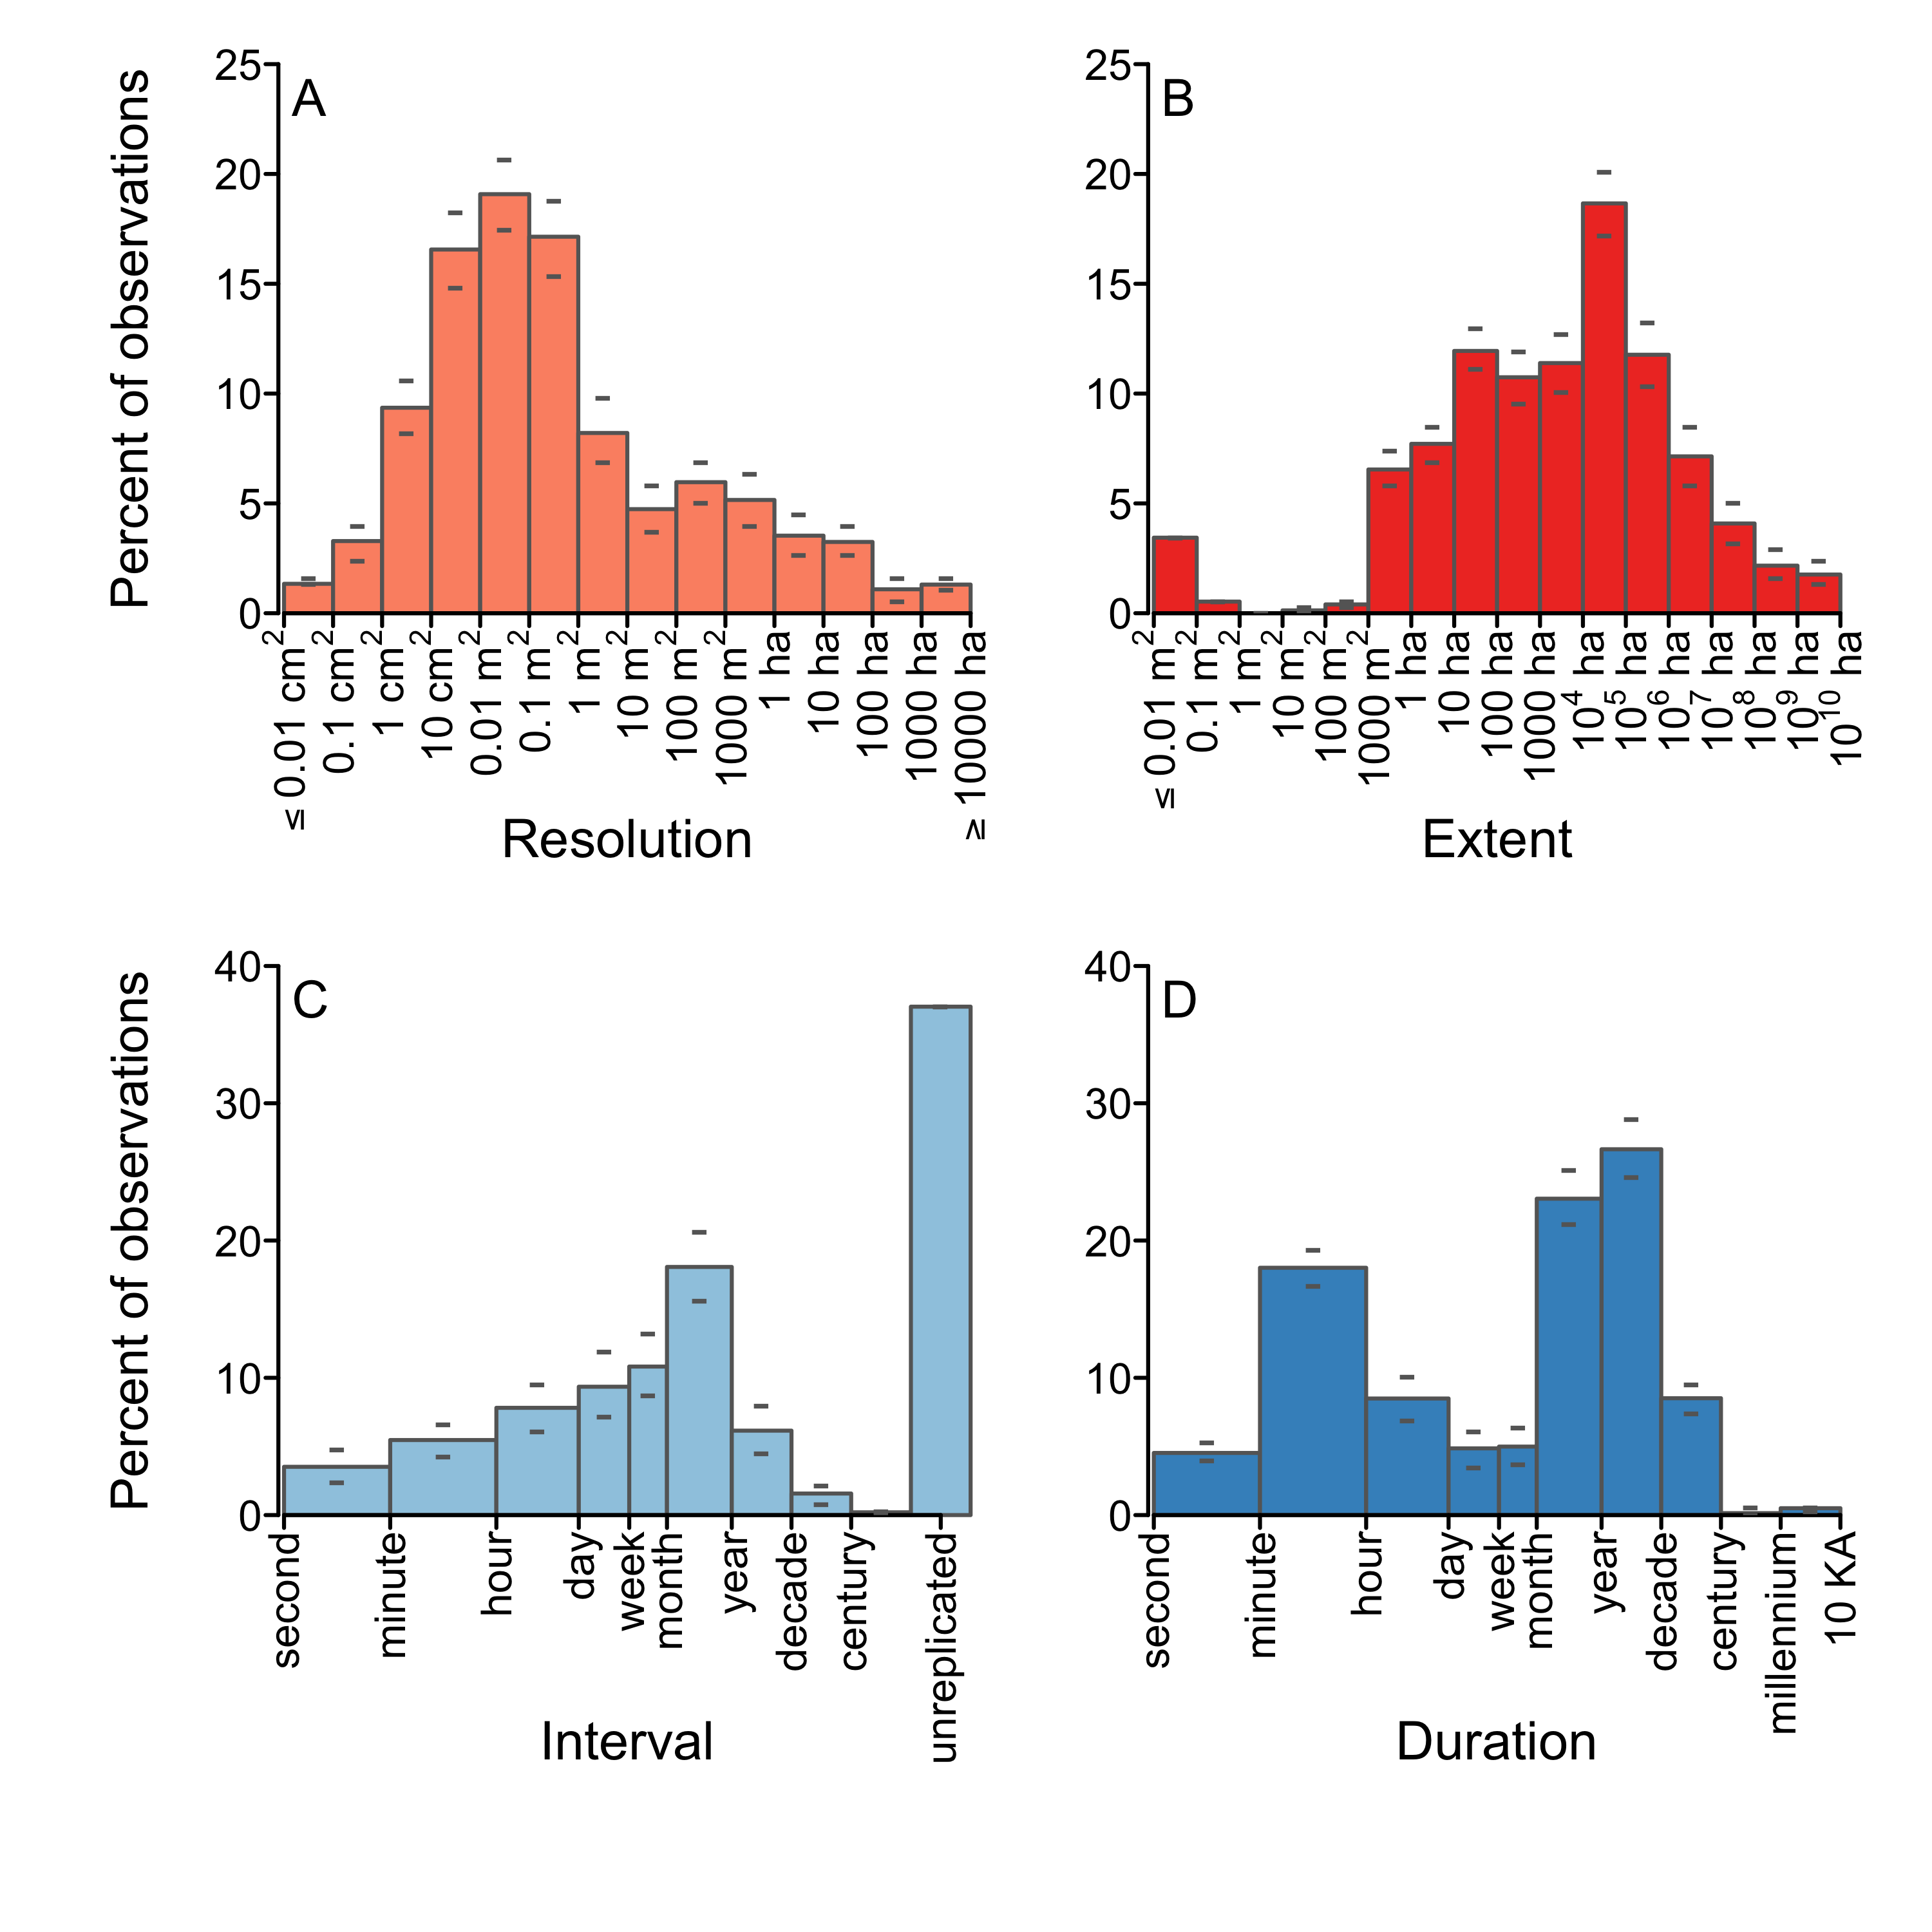
\includegraphics[width=1\textwidth]{../vignettes/figures/fig1.png}
\vspace{-0.15 cm}
\caption{Histograms of the resolution (A), extent (B), interval (C), and duration (D) of observations collected from the surveyed ecological studies. Bars represent the average percentages for each bin realized after 1000 perturbed resamples, while grey bars indicate the 95\% confidence interval. Bar widths in C-D indicate differences in scale between x-axis labels. The grey vertical line in D indicates that the majority ($>$95\%) of observations of $\leq$1 day duration were temporally unreplicated.}
\label{afoto1}
\end{figure}


\begin{figure}[!ht]
%\begin{wrapfigure}{c}{1\textwidth}
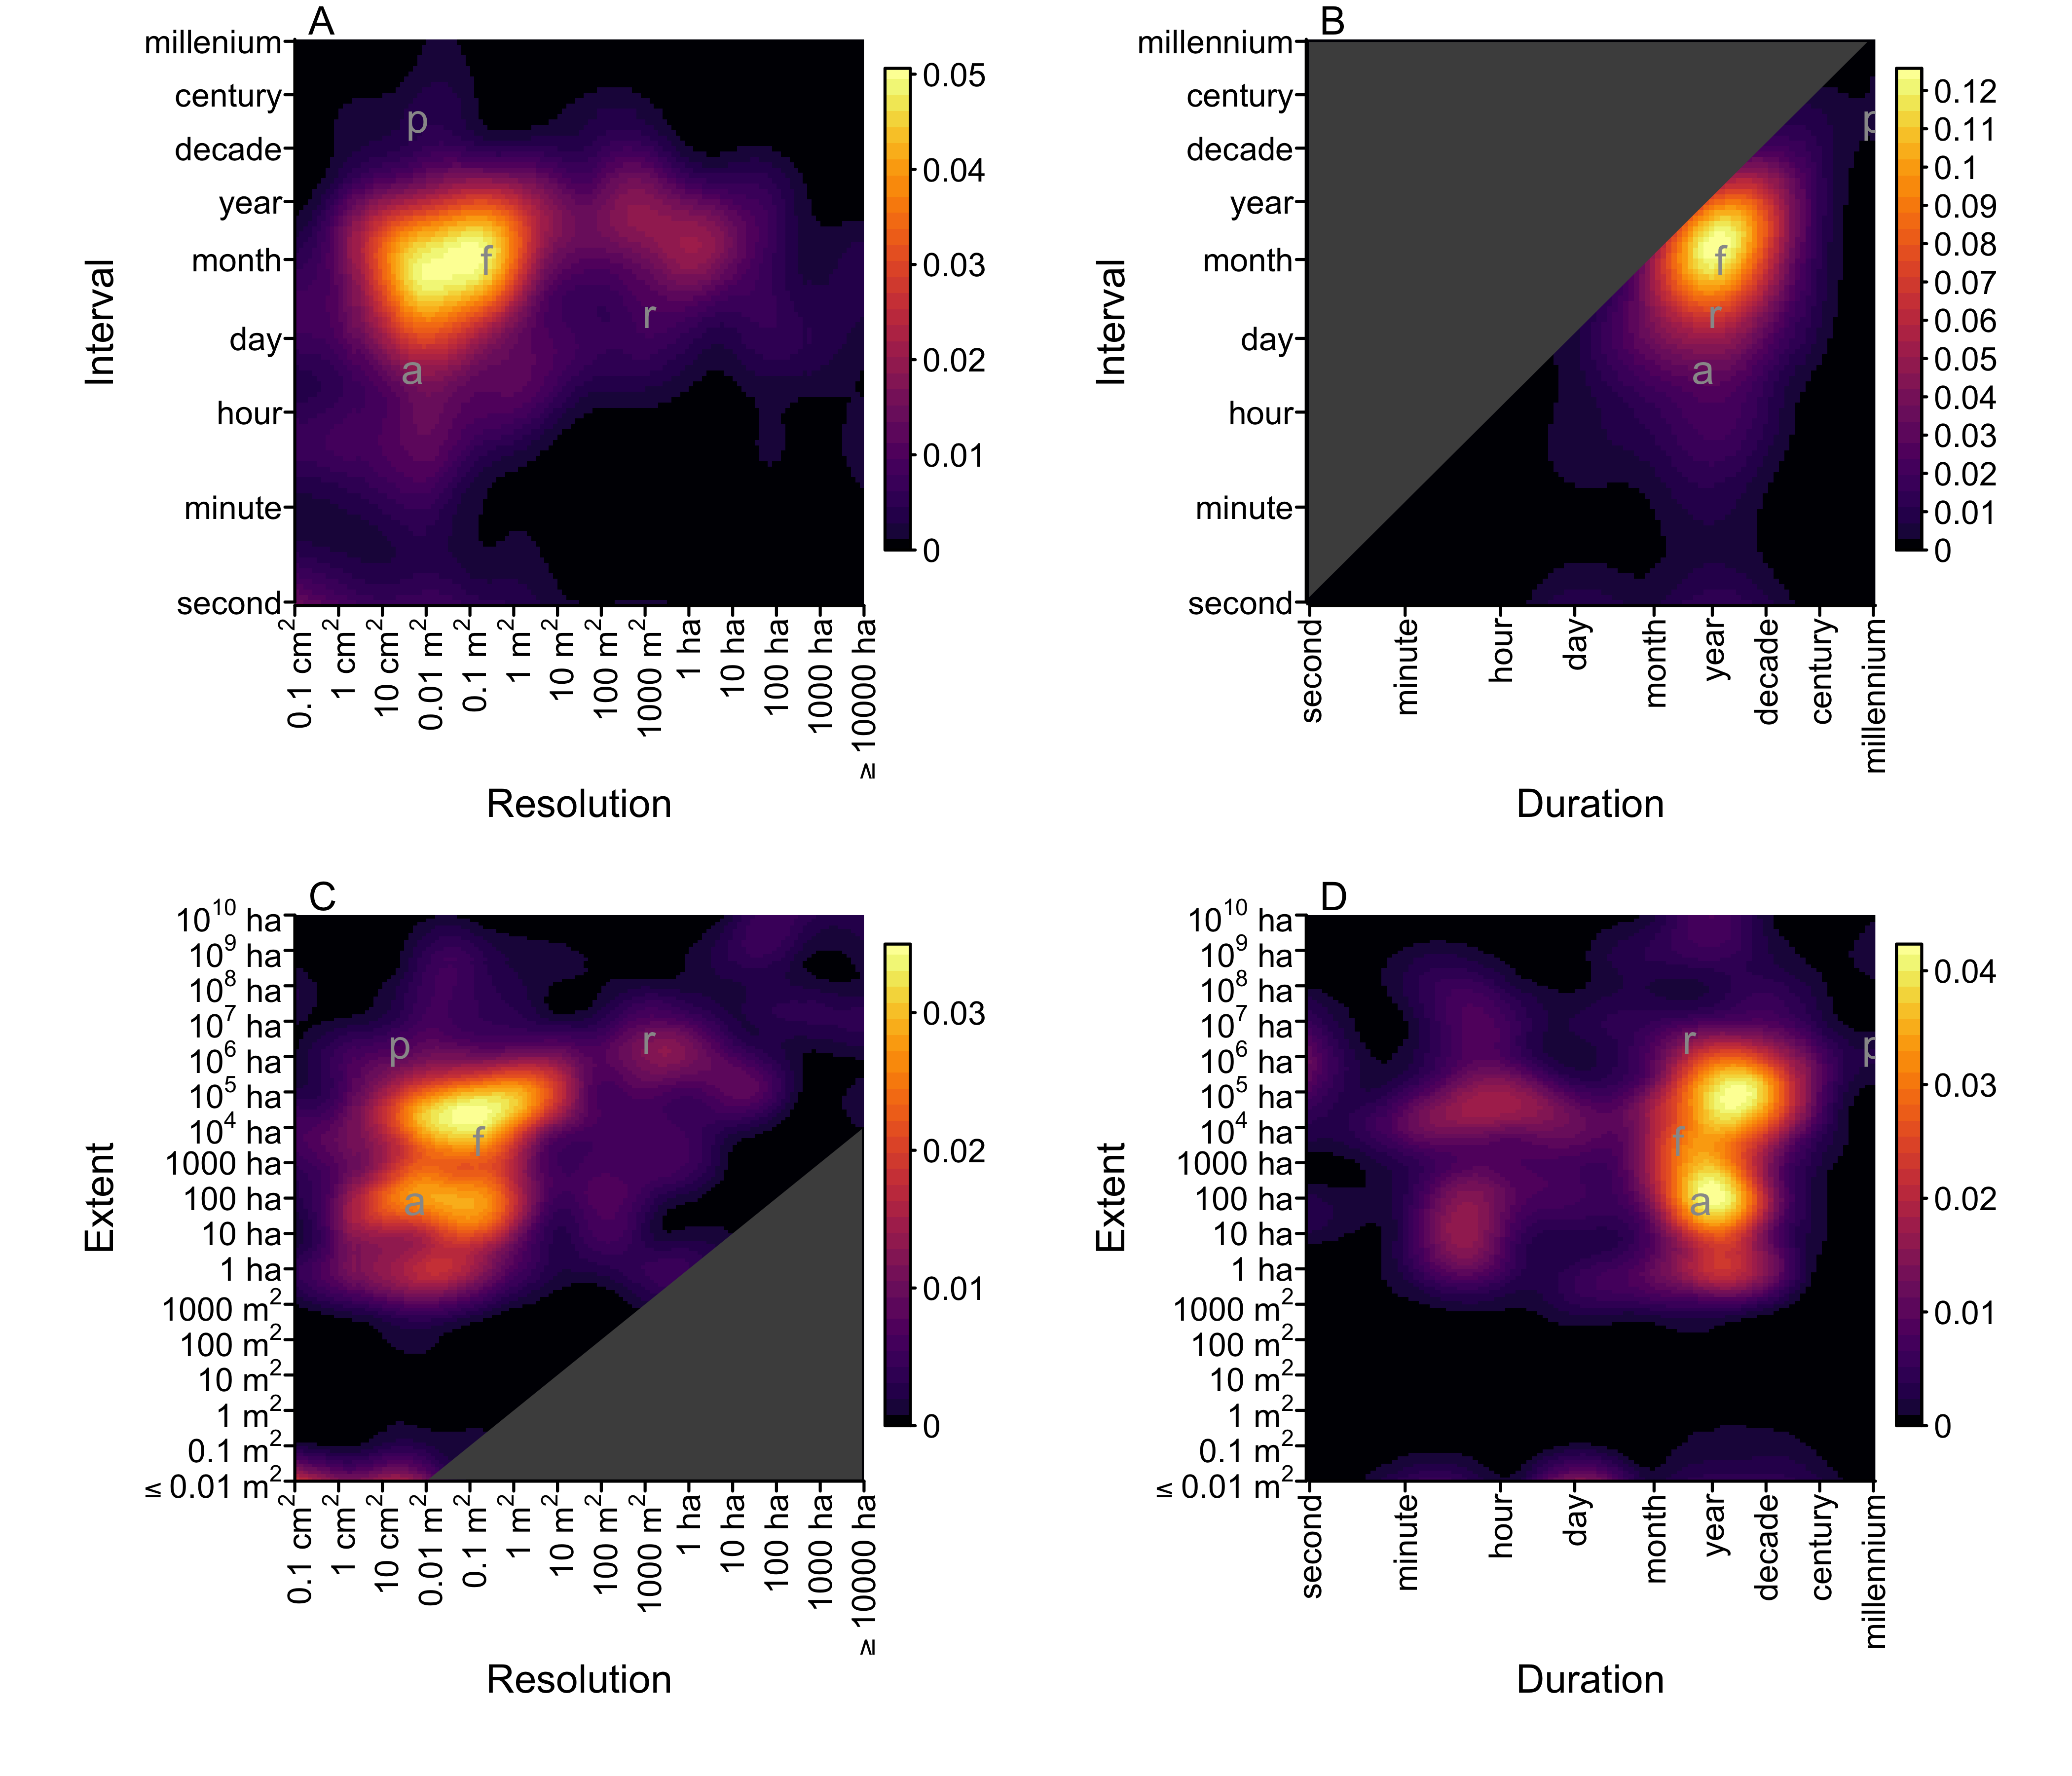
\includegraphics[width=1\textwidth]{../vignettes/figures/fig2.png}
\vspace{-0.15 cm}
\caption{Kernel density estimates of observational densities within the domains defined by A) interval and resolution (of temporally replicated observations only), B) duration and extent, C) resolution and extent, and D) interval and duration (of temporally replicated observations). Density estimates were applied to the log-transformed values of each observational dimension, and density estimates are rescaled to represent percentages. Letters in the plots denote the median values of different observational methods (f=field observations; a = automated sensing; r = remote sensing; p = paleo-observations). The grey shaded areas represent physically impossible domains (intervals greater than duration and resolutions greater than extent). Density values below the lower 3rd percentile fall within the darkest portion of the color gradient.}
\label{afoto1}
\end{figure}

\begin{figure}[ht]
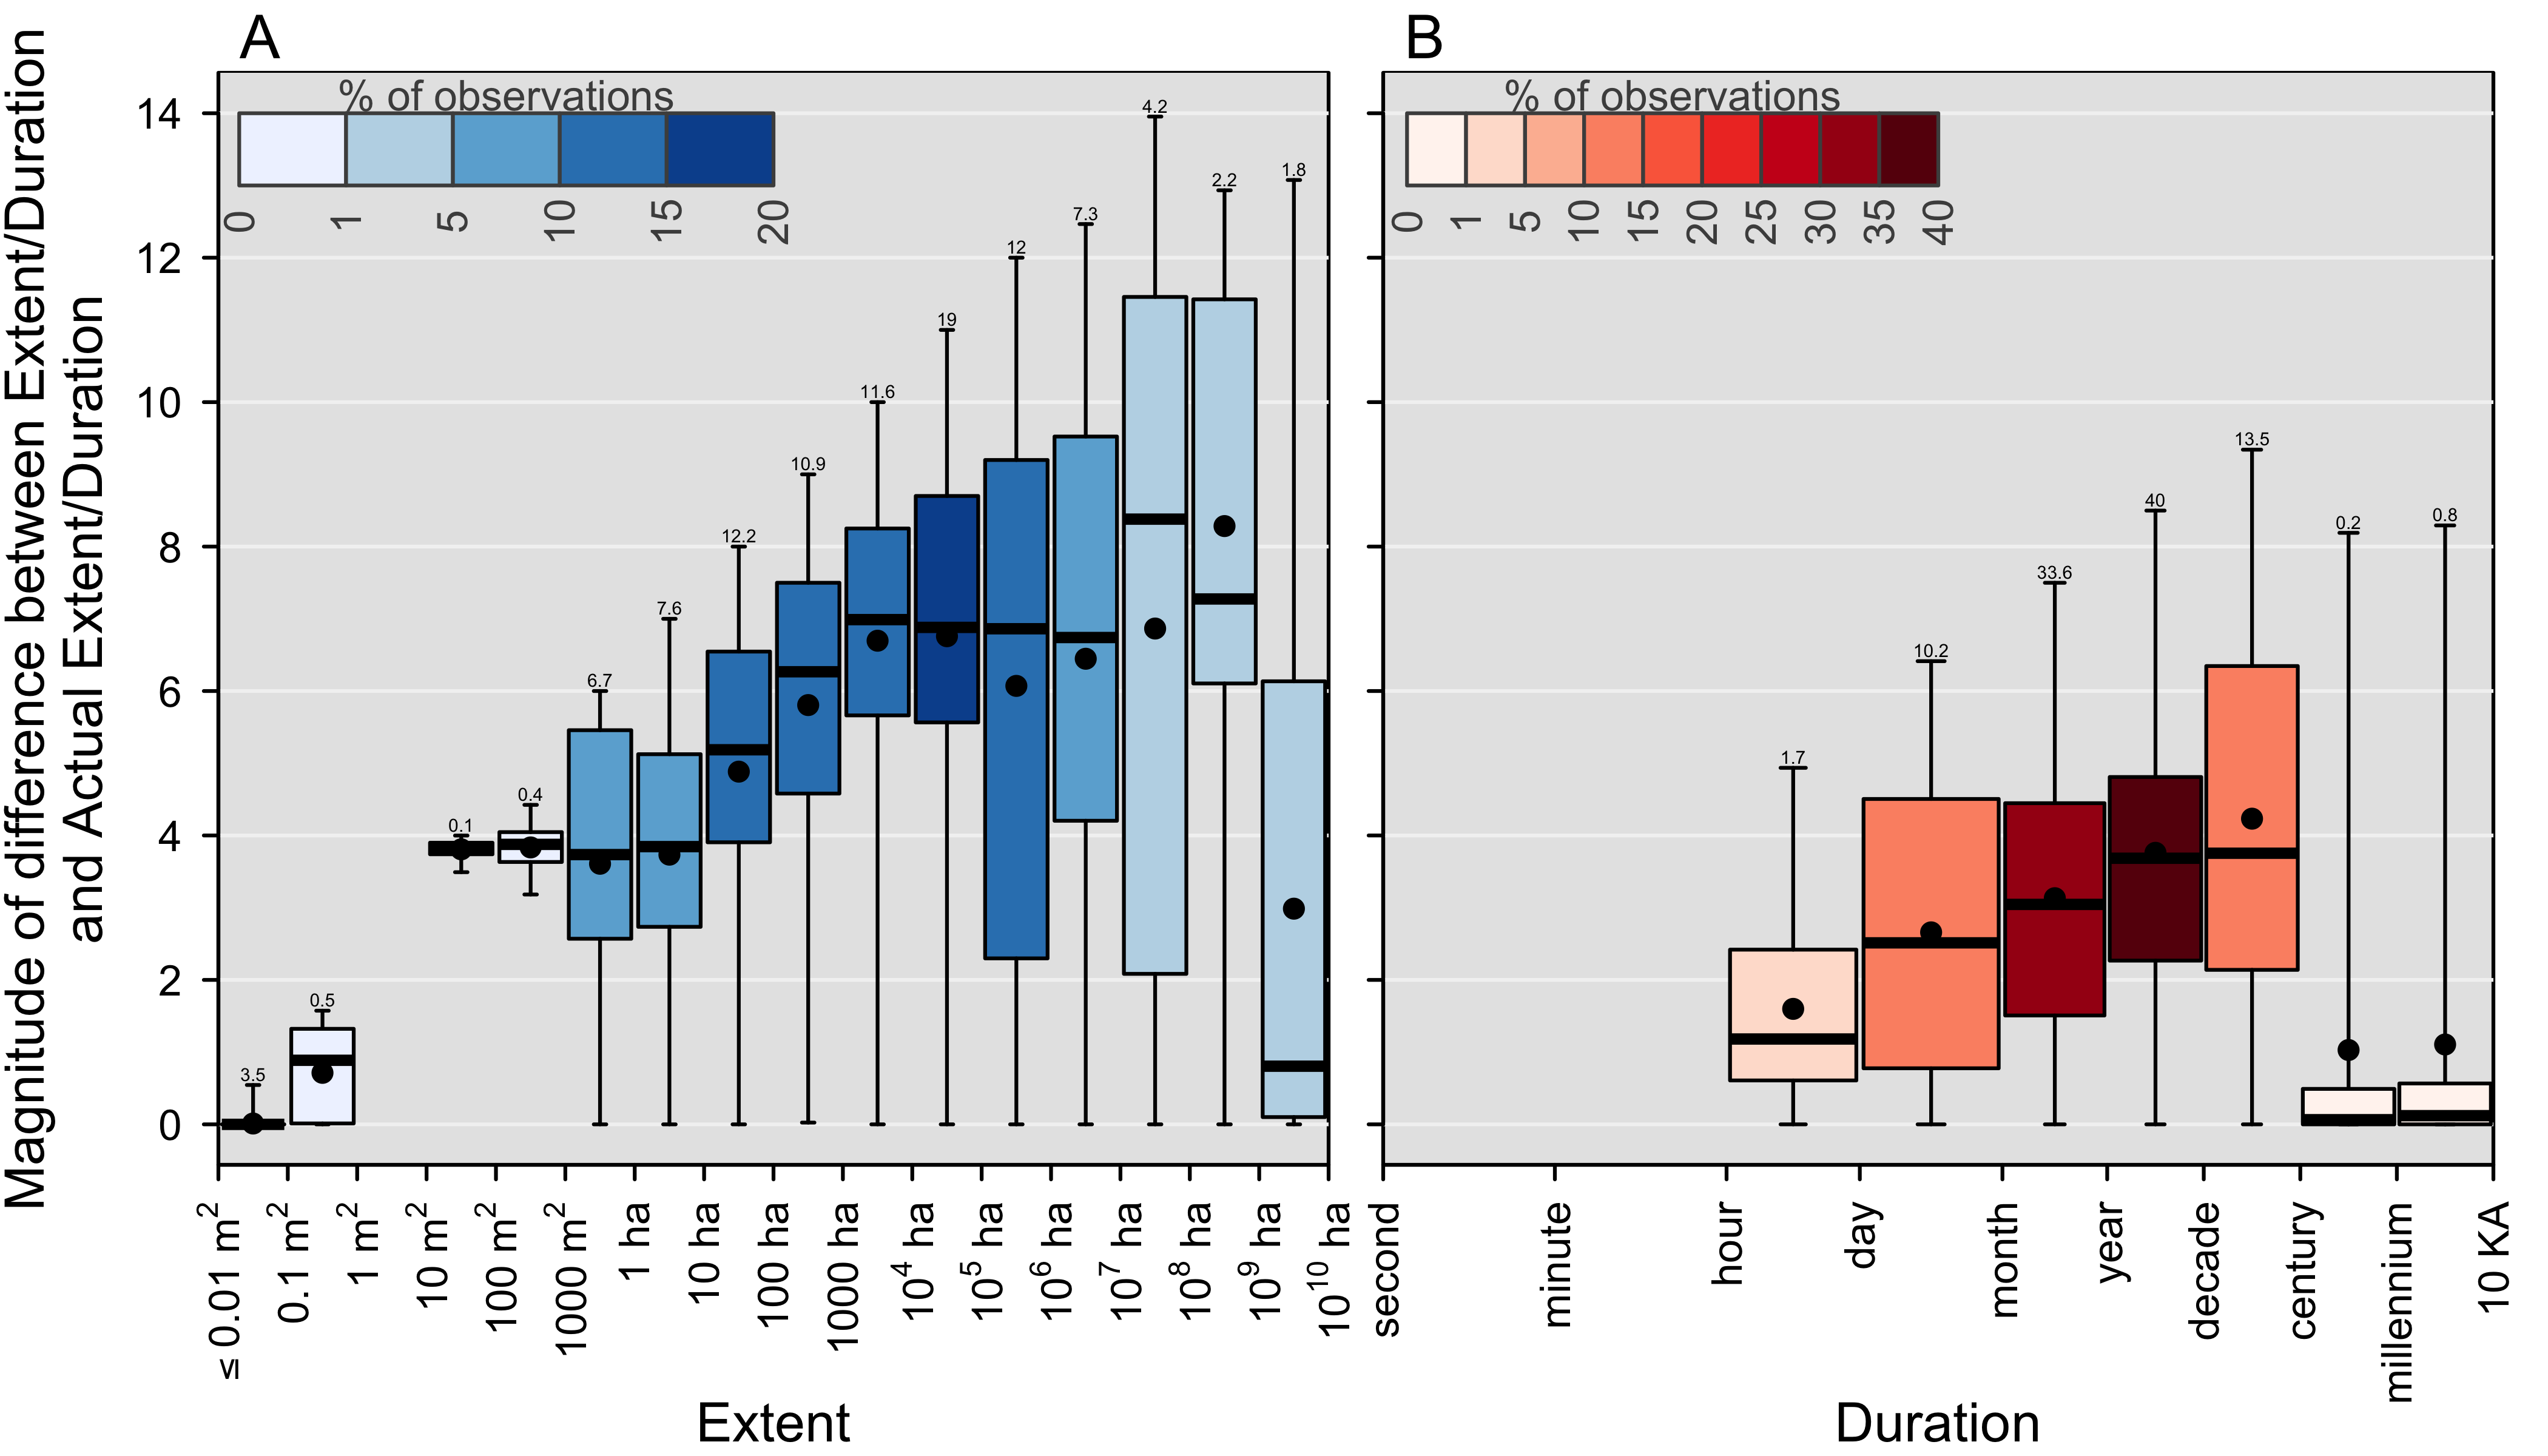
\includegraphics[width=1\textwidth]{../vignettes/figures/fig3.png}
\vspace{-0.2 cm}
\caption{The difference between extent and \emph{actual} extent (the summed area of spatial replicates) (A) and duration and \emph{actual} duration (the summed sampling duration across temporal replicates) (B). Difference values are expressed in terms of how many orders of magnitude larger (or longer) extent (duration) is than actual extent (actual duration), and are summarized (as box plots, with circle in box representing the mean and line the median) in bins representing increasing scales of actual extent/duration.  The percentages of observations falling within each bin are indicated by the color of the inter-quartile and the numeric value above the upper whisker. The grey vertical line in D indicates that the majority ($>$95\%) of observations of $\leq$1 day duration were temporally unreplicated.}
\label{afoto1}
\end{figure}


\end{document}




















